The functionality and performance of the RON image and our simple Ruby-RON
implementation where tested in the network shown in
\cref{fig:ladybug-net-ron}. To that end, we tried killing a link in the
network, after it had reached its steady state, and monitored traffic
between the terminal nodes to measure the perceived network outage
time. The experiment was also repeated for the case where no RON was
utilised.

\begin{figure}
  \centering
  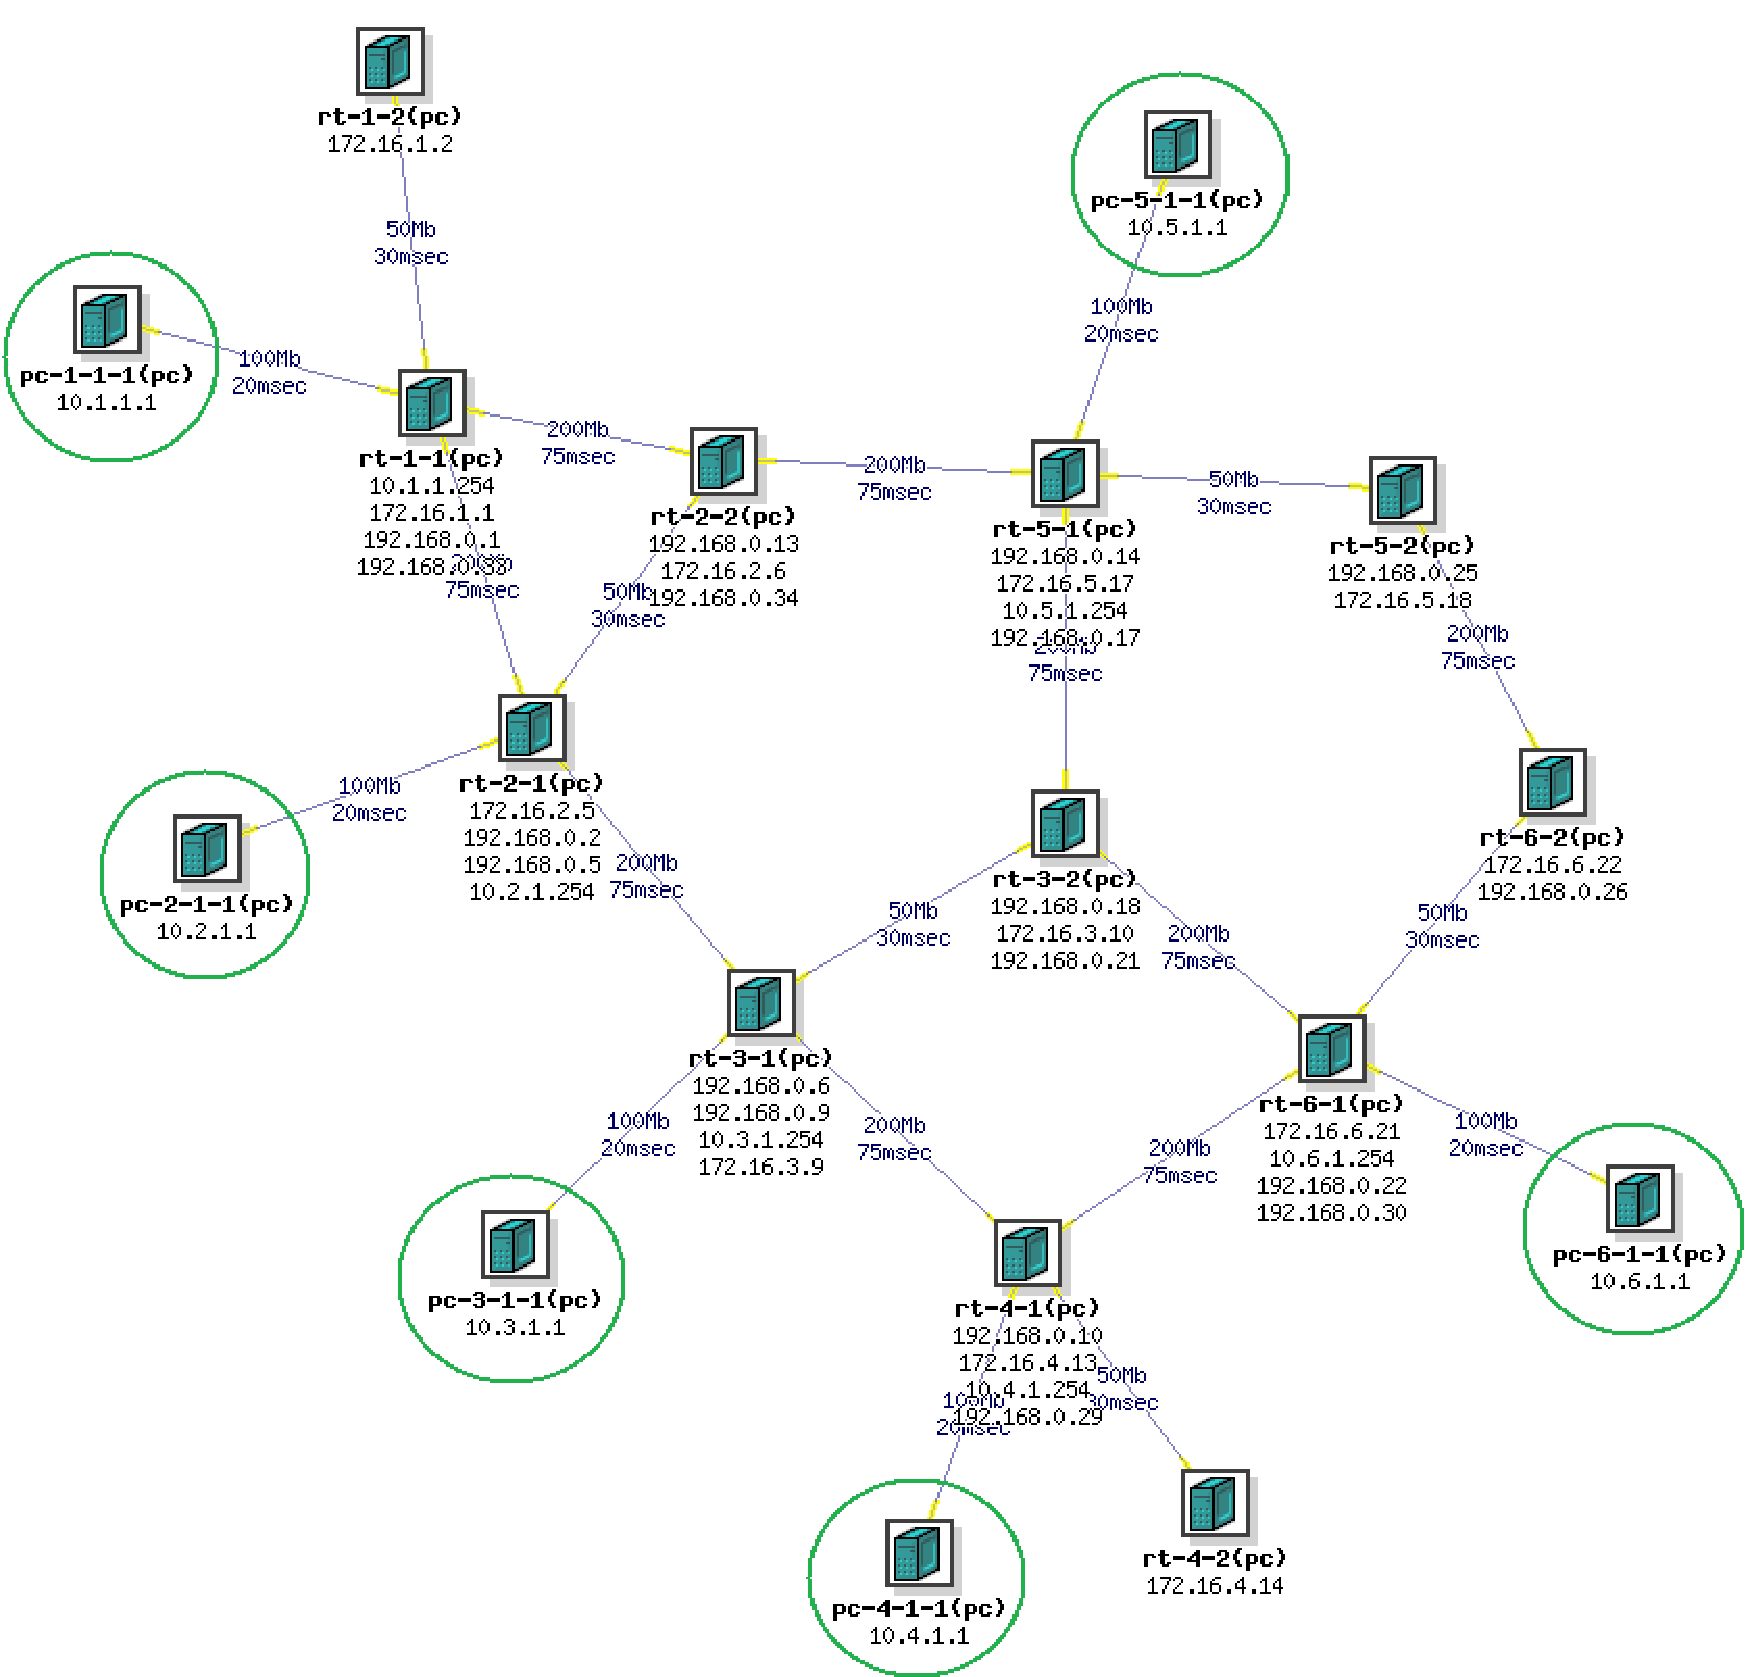
\includegraphics[width=\linewidth]{ladybug-net-ron}
  \caption{The testing network. The terminal nodes (i.e.\ the ones that
    form the overlay network) are circled.}
  \label{fig:ladybug-net-ron}
\end{figure}

As can be seen in \cref{fig:perf-ladybug}, the simple lightweight Ruby
application was able to provide a significant reduction in perceived
outages and maximized resiliency in a large network with six RON nodes.
\Cref{fig:perf-ladybug} also shows that our network topology was of
sufficient size to generate significant BGP convergence delays during link
failures.  Finally, our testing revealed that the current port of the
original RON code seems to provide no improvement in performance or fault
tolerance.

\begin{figure}
  \centering
  {\large \bfseries \sffamily Network Resiliency}
  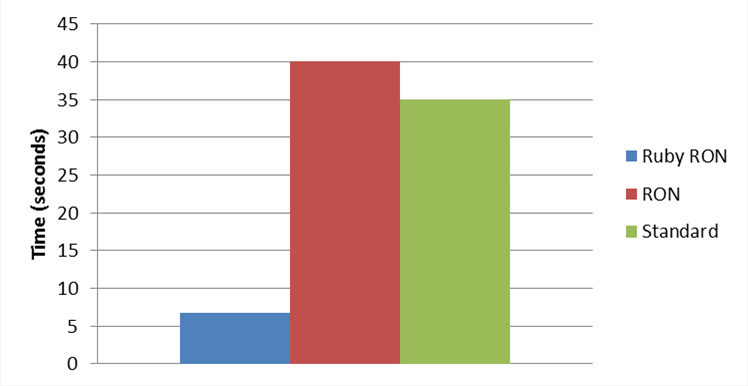
\includegraphics[width=0.8\linewidth]{route-outages-notitle}
  \caption{Average routing outage intervals after killing a link in the
    network in \cref{fig:ladybug-net-ron}. ``Standard'' means that no
    overlay network scheme was employed.}
  \label{fig:perf-ladybug}
\end{figure}

As a disclaimer, we cannot sequester enough nodes in Emulab to fully
support a scalability test for Ruby-RON; plus, some of the computational
inefficiencies discussed in \cref{sec:ron} would likely cause a performance
decrease and RON was reported to scale well for up to 50 nodes.
Additionally, we still have doubts about the functionality of our current
RON port and do not feel this performance reflects its actual capabilities,
especially since it doesn't match a large amount of published test data.


%%% Local Variables: 
%%% mode: latex
%%% TeX-master: "project-cps214"
%%% End: 

%  LocalWords:  Emulab
